\chapter{Основы}
\label{chap:basics}

\epigraph{Трейси: Я не знал, что ты была там.\\
Зоуи: В каком-то смысле. Невидимость — ты, вероятно, слышал о ней.\\
Трейси: Не думаю, что это было в базовом курсе.
}{Из 14-го эпизода <<Firefly>>}



\section{Некоторые базовые понятия в вычислениях}

\section{Асимптотическая нотация}
\subsection{Это какая-то китайская грамота!}
\subsection{Основные термины и правила}
\subsection{Take the Asymptotics for a Spin }
\subsection{Three Important Cases}
\subsection{Эмпирическая оценка алгоритмов}
\label{sec:empirical-evaluation}

В этой книге описывается\textit{ проектирование алгоритмов} (и тесно связанный с ним\textit{ анализ алгоритмов}). Но в разработке есть также и другой немаловажный процесс, жизненно необходимый при создании крупных реальных проектов, это — \textit{оптимизация алгоритмов}, искусство их \textit{эффективной реализации}. С точки зрения такого разделения, проектирование алгоритма можно рассматривать как способ достижения низкой асимптотической сложности алгоритма (с помощью разработки эффективного алгоритма), а оптимизацию — как уменьшение констант, скрытых в этой асимптотике.

Хотя я могу дать несколько советов по алгоритмам проектирования в Python, сложно угадать, какие именно хитрости и уловки дадут вам лучшую производительность в конкретной задаче, над которой вы работаете, или для вашего оборудования и версии Python. (Асимптотики используются как раз для того, чтобы не было нужды прибегать к таким вещам). Вообще, в некоторых случаях хитрости могут вовсе не потребоваться, потому что ваша программа и так достаточно быстра. Самое простое, что вы можете сделать в большинстве случаев, это просто пробовать и смотреть. Если у вас \textit{есть идея} какого-то хака, то просто опробуйте ее! Реализуйте свою хитрость и запустите несколько тестов. Есть ли улучшения? А если это изменение делает ваш код менее читаемым, а прирост производительности мал, то подумайте — стоит ли оно того?

\noindent\fbox{\parbox{\textwidth}{Этот раздел рассказывает об оценке ваших алгоритмов, а не об их оптимизации. В приложении \ref{app:A} есть несколько советов по ускорению ваших программ на Python.}}

\unmarkednote{Тестовая заметка}

Хотя теоретические аспекты так называемой экспериментальной алгоритмики (то есть, экспериментальной оценки алгоритмов и их реализации) и выходят за рамки этой книги, я дам вам несколько практических советов, которые могут быть весьма полезны.

\subsubsection*{Совет 1. Если возможно, то не беспокойтесь об этом}

Беспокойство об асимптотической сложности может быть очень полезным. Иногда \textit{решение} задачи из-за сложности на практике может \textit{перестать} быть таковым. Однако, постоянные константы в асимптотике часто совсем не критичны. Попробуйте простую реализацию алгоритма для начала, и убедитесь, что она работает стабильно. (В принципе, вы можете сначала попробовать примитивный алгоритм. Как писал гуру программирования Кен Томпсон: «Когда вы в затруднении, используйте перебор вариантов». Перебор вариантов в алгоритмах обычно означает попытку попробовать каждое из возможных решений, при этом временные затраты будут безумными!) Если она работает — не трогайте ее.

\subsubsection*{Совет 2. Для измерения времени работы используйте \texttt{timeit}}

Модуль \texttt{timeit} предназначен для измерения времени работы. Хотя для получения действительно надежных данных вам потребуется выполнить кучу работы, для практических целей timeit вполне сгодится. Например:

\begin{lstlisting}
>>> import timeit
>>> timeit.timeit("x = 2 + 2")
0.034976959228515625
>>> timeit.timeit("x = sum(range(10))")
0.92387008666992188
\end{lstlisting}

Модуль timeit можно использовать прямо из командной строки, например:

\begin{lstlisting}
python -m timeit -s"import mymodule as m" "m.myfunction()"
\end{lstlisting}

Существует кое-что, с чем вы должны быть осторожны при использовании \texttt{timeit}: побочные эффекты, которые будут влиять на повторное исполнение \texttt{timeit}. Функция \texttt{timeit} будет запускать ваш код несколько раз, чтобы увеличить точность, и если прошлые запуски влияют на последующие, то вы окажетесь в затруднительном положении. Например, если вы измеряете скорость выполнения чего-то вроде \texttt{mylist.sort()}, список будет отсортирован только \textit{в первый раз}. Во время остальных тысяч запусков список уже будет отсортированным и это даст нереально маленький результат.

Больше информации об этом модуле и о том, как он работает, можно найти в документации стандартной библиотеки Python.

\subsubsection*{Совет 3. Чтобы найти узкие места, используйте профайлер}

Часто, для того чтобы понять, какие части программы требуют оптимизации, делаются разные догадки и предположения. Такие предположения нередко оказываются ошибочными. Вместо того, чтобы гадать, воспользуйтесь профайлером. В стандартной поставке Python идет несколько профайлеров, но рекомендуется использовать \texttt{cProfile}. Им так же легко пользоваться, как \texttt{timeit}, но он дает больше подробной информации о том, на что тратится время при выполнении программы. Если основная функция вашей программы называется main, вы можете использовать профайлер следующим образом:

\begin{lstlisting}
import cProfile
cProfile.run('main()')
\end{lstlisting}

Такой код выведет отчет о времени работы различных функций программы. Если в вашей системе нет модуля \texttt{cProfile}, используйте \texttt{profile} вместо него. Больше информации об этих модулях можно найти в документации. Если же вам не так интересны детали \textit{реализации}, а просто нужно оценить поведение \textit{алгоритма} на конкретном наборе данных, воспользуйтесь модулем \texttt{trace} из стандартной библиотеки. С его помощью можно посчитать, сколько раз будут выполнены то или иное выражение или вызов в программе.

\subsubsection*{Совет 4. Показывайте результаты графически}

Визуализация может стать прекрасным способом, чтобы понять что к чему. Для исследования производительности часто применяются \textit{графики} (например, для оценки связи количества данных и времени исполнения) и диаграммы типа \textit{<<ящик с усами>>}, отображающие распределение временных затрат при нескольких запусках. Примеры можно увидеть на рисунке \ref{fig:evaluation-diagrams}.

\begin{figure}[h]
	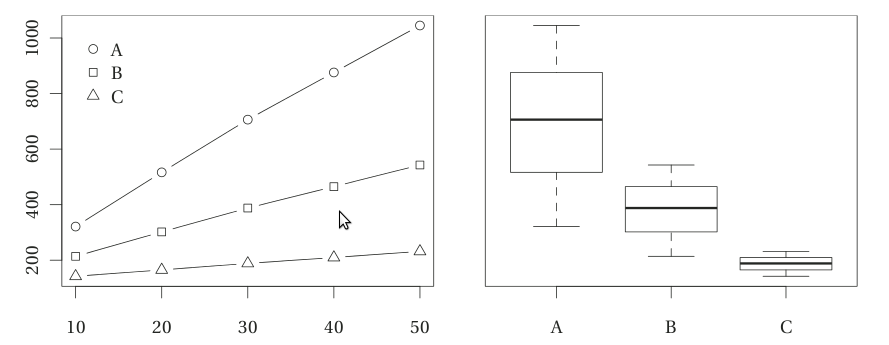
\includegraphics[width=\textwidth]{img/2-2.png}
	\caption{Визуализация времени работы для программ A, B и C и размеров данных 10 "--- 50}
	\label{fig:evaluation-diagrams}
\end{figure}

Отличная библиотека для построения графиков и диаграмм из Python "--- matplotlib (можно взять на http://matplotlib.sf.net).

\subsubsection*{Совет 5. Будьте внимательны в выводах, основанных на сравнении времени работы}

Этот совет довольно расплывчатый, потому что существует много ловушек, в которые можно попасть, делая выводы о том, какой способ лучше, на основании сравнения времени работы. Во-первых, любая разница, которую вы видите, может определяться случайностью. Если вы используете специальные инструменты вроде \texttt{timeit}, риск такой ситуации меньше, потому что они повторяют измерение времени вычисления выражения несколько раз (или даже повторяют весь замер несколько раз, выбирая лучший результат). Таким образом, всегда будут случайные погрешности и если разница между двумя реализациями не превышает некоторой погрешности, нельзя сказать, что эти реализации различаются (хотя и то, что они одинаковы, тоже \textit{нельзя} утверждать).

\noindent\fbox{\parbox{\textwidth}{Если вам нужно сделать выводы быстро, можно воспользоваться методом проверки статистических гипотез. Однако, на практике, если различия действительно очень малы, то, вероятно, неважно, какую реализацию вы выберете, так что используйте ту, что больше нравится.}}

Проблема усложняется, если вы сравниваете больше двух реализаций. Количество пар для сравнения увеличивается пропорционально \textit{квадрату} количества сравниваемых версий, \textit{сильно} увеличивая вероятность того, что как минимум две из версий будут казаться слегка различными. (Это называется проблемой \textit{множественного сравнения}). Существуют статистические решения этой проблемы, но самый простой способ "--- повторить эксперимент с двумя подозрительными версиями. Возможно, потребуется сделать это несколько раз. Они по-прежнему выглядят похожими?

Во-вторых, есть несколько моментов, на которые нужно обращать внимание при сравнении средних величин. Как минимум, вы должны сравнивать средние значения реального времени работы. Обычно, чтобы получить показательные числа при измерении производительности, время работы каждой программы нормируется делением на время выполнения какого-нибудь стандартного, простого алгоритма. Действительно, это может быть полезным, но в ряде случаев сделает бессмысленными результаты замеров. Несколько полезных указаний на эту тему можно найти в статье <<How not to lie with statistics: The correct way to summarize benchmark results>> Fleming и Wallace. Также можно почитать Bast и Weber <<Don't compare averages>>, или более новую статью Citron и др. <<The harmonic or geometric mean: does it really matter?>>.

И в-третьих, возможно, ваши выводы нельзя обобщать. Подобные измерения на другом наборе входных данных и на другом железе могут дать другие результаты. Если кто-то будет пользоваться результаты ваших измерений, \textit{необходимо последовательно задокументировать}, каким образом вы их получили.

\subsubsection*{Совет 6. Будьте осторожны, делая выводы об асимптотике из экспериментов}

Если вы хотите что-то сказать окончательно об асимптотике алгоритма, то необходимо проанализировать ее, как описано ранее в этой главе. Эксперименты могут дать вам намеки, но они очевидно проводятся на конечных наборах данных, а асимптотика "--- это то, что происходит при сколь угодно больших размерах данных. С другой стороны, если только вы не работаете в академической сфере, \textit{цель} асимптотического анализа "--- сделать какой-то вывод о поведении алгоритма, реализованного конкретным способом и запущенного на определенном наборе данных, а это значит, что измерения \textit{должны быть} соответствующими.

Предположим, вы \textit{предполагаете}, что алгоритм работает с квадратичной сложностью, но вы не можете окончательно доказать это. Можете ли вы использовать эксперименты для доказательства вашего предположения? Как уже говорилось, эксперименты (и оптимизация алгоритмов) имеют дело в основном с постоянными коэффициентами, но \textit{выход есть}. Основной проблемой является то, что ваша гипотеза на самом деле непроверяема экспериментально. Если вы утверждаете, что алгоритм имеет сложность $O(n^2)$, то данные не могут это ни подтвердить, ни опровергнуть. Тем не менее, если вы сделаете вашу гипотезу более \textit{конкретной}, то она станет проверяемой. Вы могли бы, например, основываясь на некоторых данных положить, что время работы программы никогда не будет превышать $0.24n^2+0.1n+0.03$ секунд в вашем окружении. Это проверяемая (точнее, \textit{опровергаемая}) гипотеза. Если вы сделали множество измерений, но так и не можете найти контр-примеры, значит ваша гипотеза может быть верна. А это уже и подтверждает гипотезу о квадратичной сложности алгоритма.

\section{Реализация графов и деревьев }
\label{sec:implementing-graphs-and-trees}
Первая задача из главы \ref{chap:intro}, в которой нам требовалось объехать Швецию и Китай, была примером задачи, которая может быть решена с помощью одного из мощнейших инструментов "--- с помощью \textit{графов}. Часто, если вы можете определить, что решаете задачу на графы, вы по-крайней мере на полпути к решению. А если ваши данные можно каким-либо образом представить как \textit{деревья}, у вас есть все шансы построить действительно \textit{эффективное} решение.

Графами можно представить любую структуру или систему, от транспортной сети до сети передачи данных и от взаимодействия белков в ядре клетке до связей между людьми в Интернете.
Ваши графы могут стать еще полезнее, если вы добавите в них дополнительные данные вроде \textit{весов} или \textit{расстояний}, что даст возможность описывать такие разнообразные проблемы как игру в шахматы или определение подходящей работы для человека в соответствии с его способностями.
Деревья — это просто особый вид графов, так что большинство алгоритмов и представлений графов сработают и для них.
Однако, из-за их особых свойств (связанность и отсутствие циклов), можно применить специальные (и весьма простые) версии алгоритмов и представлений.
На практике в некоторых случаях встречаются структуры (такие как XML-документы или иерархия каталогов), которые могут быть представлены в виде деревьев\footnote{С учетом атрибутов IDREF и символьных ссылок XML-документы и иерархия каталогов становятся собственно графами.}. На самом деле эти <<некоторые>> случаи довольно-таки общие.

Если вы забыли терминологию (или ее и не знали), почитайте приложение \ref{app:graph-theory}, <<Терминология теории графов>>. Здесь же опишем основные моменты:
\begin{itemize}
\item Граф $G = (V, E)$ состоит из \textit{вершин}, $V$, и \textit{ребер} между ними, $E$. Если ребра имеют направление, то граф называется \textit{направленным}.
\item Вершины, связанные ребром, называются \textit{смежными}. Соединяющее две вершины ребро называется \textit{инцидентным} с ними. Вершины, смежные с $v$ называются \textit{соседними} с $v$.
\item \textit{Подграф} графа $G = (V,E)$ состоит из подмножества $V$ и подмножества $E$. \textit{Путь} в графе "--- это подграф, вершины которого соединены ребрами последовательно, причем каждая вершина включена только один раз. \textit{Цикл} — это то же самое, что и путь, только последнее его ребро связывает последнюю вершину с первой.
\item Если каждому ребру в $G$ будет сопоставлено определенное значение (\textit{вес}), то $G$ будет называться \textit{взвешенным} графом. \textit{Длина} пути или цикла — это сумма всех весов его ребер или, для невзвешенных графов, просто количество ребер.
\item \textit{Лесом} называется граф без циклов, а связанный граф — это \textit{дерево}. Иными словами, лес состоит из одного или многих деревьев.
\end{itemize}

Описание задачи в терминах графов является довольно абстрактным, так что если вам нужно реализовать решение, вы должны представить графы в виде каких-либо структур данных.


\subsection{Adjacency Lists and the Like}
\subsection{Adjacency Matrices}
\subsection{Implementing Trees}
\subsection{A Multitude of Representations}

\section{Beware of Black Boxes}
\subsection{Hidden Squares}
\subsection{The Trouble with Floats}
\section{Summary}
\section{If You’re Curious…}
\section{Exercises}
\section{References}





%%% Local Variables: 
%%% mode: latex
%%% TeX-master: "mapl"
%%% End: 
